\fancyfoot[RE,LO]{Autor: Julia Gartner}

\section {Mobile Applications} \label {MobileApplications}

\subsection {Einleitung} \label {MAEinleitung}

Eine Mobile Application, oft nur App genannt, ist Software, die auf mobilen Ger�ten verwendet werden kann. Solche Ger�te sind z.B. Smartphones, Tablets oder Smartwatches und haben meistens entweder Android oder iOS als Betriebssystem\cite{reg401}. Generell gibt es viele Anwendungen f�r mobile App wie Kommunikation, E-Commerce und Weiterbildung\cite{reg402}. In unserem Fall hat das Software Interface prim�r die Aufgabe, die mithilfe des EOGs gesammelten Daten f�r den User graphisch darzustellen. Sekund�r gibt es eine Weckerfunktion.

\subsection {Allgemeines zur Mobilapp-Entwicklung} \label {MA Allgemeines}

Wie bereits in Kapitel \ref{MAEinleitung} erw�hnt, sind die meistverbreiteten Betriebssysteme, die die Umgebung f�r Mobile Apps darstellen, iOS und Android mit einem Marktanteil von 99\% im Jahr 2018 in den USA. Mobile Apps f�r diese beiden Betriebssysteme werden jedoch nicht in der selben Sprache geschrieben. F�r Android kann in Java oder Kotlin geschrieben werden, w�hrend f�r iOS Objective-C oder Swift verwendet wird. Das ist in der Praxis oft nicht optimal, da eine Anwendung erstens in zwei verschiedenen Sprachen geschrieben werden muss und zweitens auch zwei verschiedene Anwendungen gewartet werden m�ssen\cite{reg403}. Eine L�sung f�r dieses Problem sind Hybrid Mobile App Development Frameworks. Mit diesen Frameworks k�nnen Apps in einer Sprache geschrieben werden und trotzdem auf verschiedenen Betriebssystemen laufen\cite{reg404}.\\

\begin{figure}[H]
	\centering
		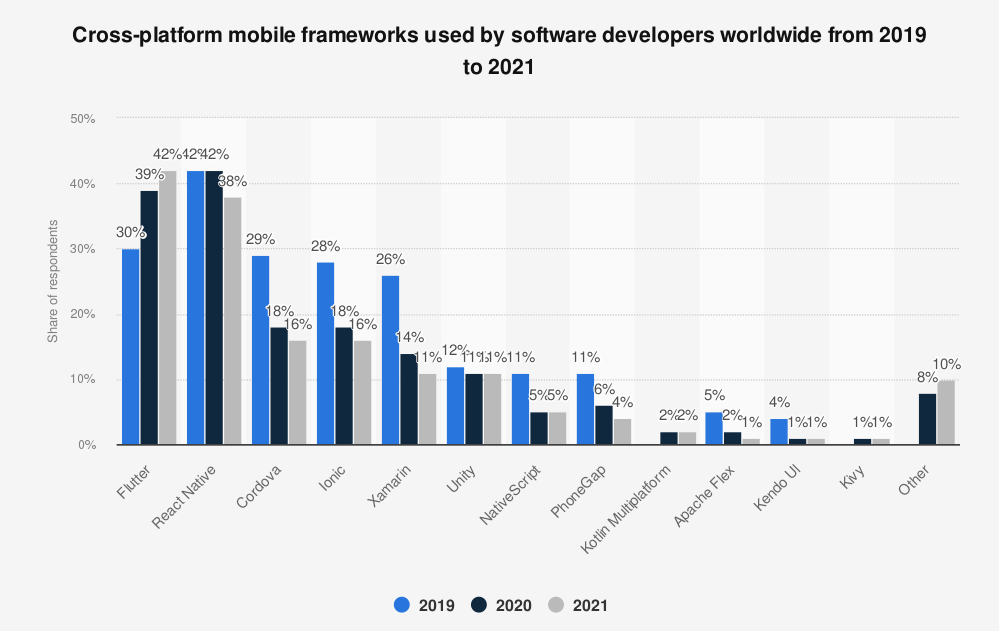
\includegraphics[width=0.9\textwidth]{Gartner/cross_platform_use_statistic.png}
	\caption{Plattform�bergreifende Mobile-Frameworks die von Softwareentwicklern weltweit verwendet werden (2019 bis 2021)\cite{reg405}}
	\label{fig:cross_platform_use_statistic}
\end{figure}

Wie in Abbildung \ref{fig:cross_platform_use_statistic} zu sehen ist, sind die zwei meist verwendeten plattform�bergreifenden Mobile-Frameworks seit 2019 Flutter und React Native, was sich immer weiter absetzt. W�hrend im Jahr 2019 das meistverwendete Framwork noch React Native war, verwenden 2021 die meisten Entwickler bereits Flutter.  \\
React Native und Flutter unterscheiden sich in mehreren Hinsichten. Zum einen wird das React Native-Framework mit JavaScript verwendet, w�hrend ein Flutter-Projekt in Dart geschrieben wird. React Native erreicht die plattformunabh�ngige Anwendung durch eine Br�cke; ein React Native-Projekt in JavaScript auf einem Android-Ger�t z.B. kommuniziert �ber diese Br�cke mit nativen Komponenten des Betriebssystems. Bei Flutter hingegen wird ein Projekt beim Kompilieren von Dart direkt zu einer nativen Sprache �bersetzt, f�r ein Ger�t ist das also nicht zu unterscheiden von einer nativen App\cite{reg406}.

\subsubsection {Entwicklungsumgebung} \label{}

VSCode, Android Studio Emulator

\subsection {Flussdiagramm} \label {}

\subsection {Funktionalit�t} \label {}

\subsubsection {Framework} \label {} 

Flutter, auch in Bezug auf plattformunabh�ngigkeit, Objekte, Widgets

\subsubsection {State-Management} \label{}

State, Provider

\subsubsection {Data-Fetching} \label{}

\paragraph {Clientside} \label{}

Async functions, json, post vs. get request

\paragraph {Hostside} \label{}

bisschen zu php seite

\subsubsection {Graphische Darstellung der Daten} \label{}

syncfusion flutter charts






